\documentclass[11pt,a4paper,openany]{report}
\usepackage[T1]{fontenc}
\usepackage{lmodern}
\usepackage{microtype}
\usepackage[margin=25mm]{geometry}
\usepackage{amsmath,amssymb,mathtools}
\usepackage{booktabs,longtable,tabularx,array}
\usepackage{enumitem}
\usepackage[dvipsnames]{xcolor}
\usepackage{hyperref}
\usepackage{cleveref}
\usepackage{tikz}
\usetikzlibrary{arrows.meta,positioning,calc,fit,shapes.geometric}
\usepackage{fancyhdr}
\usepackage{titlesec}
\usepackage[most]{tcolorbox}
\usepackage{listings}
\usepackage{pdfpages}
\usepackage{ragged2e}
\usepackage{lastpage}
\usepackage{seqsplit}
\definecolor{PNCSNavy}{HTML}{182A4A}
\definecolor{PNCSBlue}{HTML}{2E5B93}
\definecolor{PNCSLight}{HTML}{F3F6FA}
\definecolor{PNCSGray}{HTML}{606A78}
\hypersetup{colorlinks=true,linkcolor=PNCSBlue,urlcolor=PNCSBlue,citecolor=PNCSBlue,pdftitle={PhaseNav Natural Coding System - Current Repository Monograph},pdfauthor={Adrian Lipa}}
\titleformat{\chapter}[display]{\bfseries\color{PNCSNavy}}{\Large CHAPTER \thechapter}{8pt}{\Huge}
\titleformat{\section}{\Large\bfseries\color{PNCSNavy}}{\thesection}{0.7em}{}
\titleformat{\subsection}{\large\bfseries\color{PNCSBlue}}{\thesubsection}{0.7em}{}
\setlength{\parindent}{0pt}
\setlength{\parskip}{0.55em}
\setlength{\emergencystretch}{3em}
\setlength{\headheight}{14pt}
\pagestyle{fancy}
\fancyhf{}
\lhead{PNCS Current Repository Monograph}
\rhead{23 August 2026}
\cfoot{\thepage}
\newcommand{\Tthirtysix}{T^{36}}
\newcommand{\kappaTIR}{\kappa=\frac{\ln2}{24\pi}}
\newcommand{\sha}[1]{\texttt{\small\seqsplit{#1}}}
\newcommand{\status}[1]{\texttt{#1}}
\newtcolorbox{statusbox}[1]{colback=PNCSLight,colframe=PNCSBlue,title={#1},fonttitle=\bfseries,breakable}
\newtcolorbox{boundarybox}{colback=white,colframe=PNCSNavy,title={Boundary},fonttitle=\bfseries,breakable}
\newtcolorbox{interpbox}{colback=PNCSLight,colframe=PNCSGray,title={INTERPRETACJA},fonttitle=\bfseries,breakable}
\lstset{basicstyle=\ttfamily\small,backgroundcolor=\color{PNCSLight},frame=single,rulecolor=\color{PNCSGray},breaklines=true,columns=fullflexible}
\begin{document}
\begin{titlepage}
\centering
\vspace*{20mm}
{\Huge\bfseries\color{PNCSNavy} PhaseNav Natural\\[2mm] Coding System\\[4mm] (PNCS)\par}
\vspace{10mm}
{\LARGE A Content-Addressed 36-Dimensional\\Relational Programming and Runtime Architecture\par}
\vspace{14mm}
{\Large\bfseries Current Repository Monograph\par}
\vspace{3mm}
{\large v0.1--v0.27 release line + current v0.28 closure gate and experimental modules\par}
\vfill
{\Large Adrian Lipa\par}
\vspace{6mm}
{\large 23 August 2026\par}
\vspace{13mm}
\begin{minipage}{0.88\textwidth}
\small
\textbf{Status:} NON-NORMATIVE REPOSITORY-WIDE SYNTHESIS. The v0.26 monograph is preserved verbatim as Part I. Part II updates the document to the repository snapshot at main commit \sha{de8ccd4a6d7c32bd0a079a679416c556c5901790} and records active branch state separately from main authority. Normative authority remains with versioned specifications, registries, receipts and ledgers in the repository.
\end{minipage}
\vspace{10mm}
\href{https://github.com/AdrianLipa90/PhaseNav-Natural-Coding-System}{github.com/AdrianLipa90/PhaseNav-Natural-Coding-System}
\end{titlepage}
\pagenumbering{roman}
\chapter*{How to read this edition}
\addcontentsline{toc}{chapter}{How to read this edition}
This edition deliberately does not rewrite the previously published v0.26 core. Part I reproduces the complete 55-page v0.26 monograph exactly. Its statements about the ``current engineering frontier'' are therefore historical statements made at the v0.26 boundary. Part II is the authoritative update layer for this repository snapshot.

The update distinguishes four statuses throughout:
\begin{description}[leftmargin=35mm,style=nextline]
\item[\status{MAIN}] present on the current main tree;
\item[\status{RELEASE\_CLOSED}] a gate whose defined release scope is closed by its own receipt;
\item[\status{BRANCH}] present on a non-main Git branch and not silently promoted;
\item[\status{EXPERIMENTAL}] implemented or validated research material that explicitly does not advance the PNCS release sequence.
\end{description}
\begin{statusbox}{Current repository anchor}
Main: \sha{de8ccd4a6d7c32bd0a079a679416c556c5901790}. Current main contains both the merged PR \#16 experimental prime-temporal layer and the merged PR \#15 v0.28 release-closure implementation. The v0.28 specification still states \status{RELEASE NOT CLOSED}. The prime-temporal ledger remains \status{EXPERIMENTAL\_PURE\_CORE\_PASS}, \status{READ\_ONLY}, \status{NON\_PROMOTING}; its presence on main is not equivalent to a new PNCS release gate.
\end{statusbox}
\tableofcontents
\clearpage
\pagenumbering{arabic}
\part{Preserved PNCS core: project monograph v0.26}
\includepdf[pages=-,pagecommand={}]{PNCS_MONOGRAPH_V0_26_BASE.pdf}
\part{Current repository update}
\chapter{Current repository snapshot}

\begin{statusbox}{Snapshot}
Repository: \texttt{AdrianLipa90/PhaseNav-Natural-Coding-System}.\\
Current main: \sha{de8ccd4a6d7c32bd0a079a679416c556c5901790}.\\
Immediate main history includes PR \#16 (experimental prime-temporal layer) followed by PR \#15 (v0.28 release-closure implementation).\\
Current release-closed engineering gate: v0.27 ORCHORBITAL-coupled hydrodynamic proper-time runtime.\\
Current release-closure programme: v0.28 adversarial conformance is now present on main, but its normative spec remains \emph{release not closed}.
\end{statusbox}

The v0.26 monograph stopped at the Effect Boundary. Since that document was produced, the repository acquired three distinct layers that must not be collapsed into one release label:

\begin{enumerate}
\item the release-closed v0.27 ORCHORBITAL/hydrodynamic execution substrate on \(\Tthirtysix\);
\item the temporal-fibre optimization, whose implementation and measured validation are now present on main but whose specification retains an experimental-optimization status;
\item the experimental prime-temporal hydrodynamic coding layer, merged to main by PR \#16 but explicitly non-promoting.
\end{enumerate}

v0.28 release-closure code is now integrated on main, while its gate status remains open. Therefore repository membership is not release authority. The repository now contains both release-line code and research-line code, and the monograph must label them independently.

\section{Current main layering}
\begin{center}
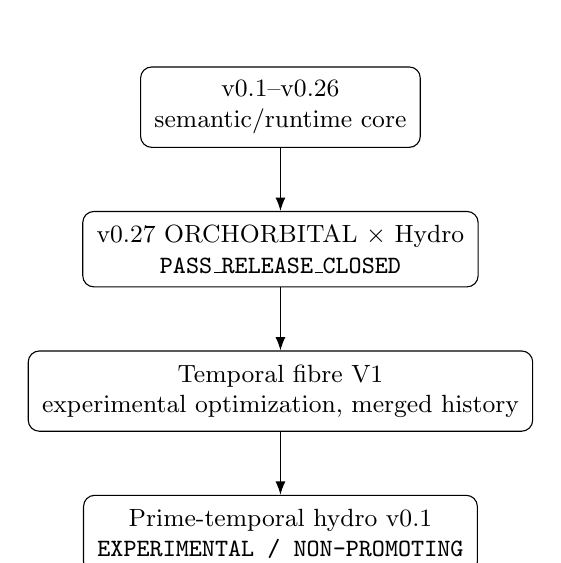
\begin{tikzpicture}[node distance=8mm,>=Latex,every node/.style={draw,rounded corners,align=center,inner sep=5pt,font=\small}]
\node (core) {v0.1--v0.26\\semantic/runtime core};
\node[below=of core] (v27) {v0.27 ORCHORBITAL $\times$ Hydro\\\status{PASS\_RELEASE\_CLOSED}};
\node[below=of v27] (tf) {Temporal fibre V1\\experimental optimization, merged history};
\node[below=of tf] (prime) {Prime-temporal hydro v0.1\\\status{EXPERIMENTAL / NON-PROMOTING}};
\draw[->] (core)--(v27); \draw[->] (v27)--(tf); \draw[->] (tf)--(prime);
\end{tikzpicture}
\end{center}

The arrows above indicate repository accumulation, not semantic authority flow. In particular, the prime-temporal module cannot route semantic execution, modify effect authority, modify the hydrodynamic lapse, or claim laboratory-time modification.

\section{Operational invariant}
The standing live-runtime invariant remains:
\[
\boxed{\text{36D operation}\longrightarrow /\texttt{dev/shm/ciel\_noema}\longrightarrow\text{live runtime authority}.}
\]
Persistent repository and Library artifacts may hydrate or verify that surface; they are not an operational substitute.

\section{Manifest status}
The root \texttt{MANIFEST.sha256.json} is currently non-authoritative and fail-closed. Its status is \status{INVALIDATED\_BY\_REPOSITORY\_LAYOUT\_CANONICALIZATION}. A complete final-tree file-byte SHA-256 manifest, repository conformance and manifest receipt remain required before a gate that depends on final-tree closure may be declared closed.

\chapter{v0.27 ORCHORBITAL-coupled hydrodynamic proper-time runtime}

\begin{statusbox}{Release status}
\status{PASS\_RELEASE\_CLOSED} for the explicitly defined v0.27 scope. The foundation receipt on main is \texttt{provenance/receipts/FOUNDATION\_STATUS\_V0\_27.json}.
\end{statusbox}

v0.27 binds the existing PNCS resident execution authority to a synchronous ORCHORBITAL and hydrodynamic phase-flow substrate. The defining invariant is that semantic execution remains exact while a separate \(\Tthirtysix\) process state evolves alongside every semantic KAKU occurrence.

\section{Coupled execution chain}
\begin{lstlisting}
resident v0.25 authority
-> exact v0.20 semantic KAKU transition
-> ORCHORBITAL Psi_t / K_ij / attractor envelope
-> T^36 hydrodynamic phase-flow / local Delta tau
-> ORCHORBITAL observables + reduction readiness
-> next exact semantic KAKU transition
-> deterministic coupled receipt
\end{lstlisting}

The semantic projection is frozen against v0.20 authority. It must preserve operator order, exact operator-vector byte SHA-256, operator bindings, program provenance, branch truth and result location.

\section{State and observables}
The base relational manifold is denoted \(M_{\rm rel}\). The geometric anchor is projective Hilbert/K\"ahler/Fubini--Study. The runtime binds thirty-six internal process modes,
\[
\Psi_t=\{o_i(t)\}_{i=1}^{36},
\]
with an explicit symmetric phase-aware coupling \(K_{ij}\).

The retained ORCHORBITAL observables include
\[
C(t),\quad \Delta=1-C,\quad \Delta_H,\quad R_H=|\Delta_H|^2,
\quad V_{\rm tot},\quad A_{\rm eff},\quad \Omega.
\]
The reduction readiness scalar remains explicit,
\[
\Omega=\lambda_1C+\lambda_2R(S,I)-\lambda_3\Delta-\lambda_4\Xi,
\qquad \texttt{reduce\_ready}\iff \Omega\ge\Omega_{\rm crit}.
\]
Reduction readiness does not select an orbital. Stable residue is emitted only after reduction plus explicit selection.

\section{Hydrodynamic phase proper time}
The substrate implemented in the current v0.27 line is
\[
N_{\rm substrate}=\operatorname{clip}\!\left(\frac{\sqrt\rho}{1+\nu_{\rm eff}}\right),
\qquad
G_{\rm eff}=\rho I+uu^T,
\]
combined with the explicitly bound ORCH subjective-time factor,
\[
g_{\rm combined}=\operatorname{clip}(N_{\rm substrate}g_{\rm orb}),
\qquad
\Delta\tau=\Delta t\,g_{\rm combined}.
\]
The Foundation Pack relation
\[
\Delta\tau_i(k)=\Delta t\,g(r_i,C_i,\Delta_i,m_i,A_i)
\]
is preserved, but the Foundation Pack does not freeze a unique closed form for \(g\). PNCS therefore uses a content-addressed parametric family with receipt-bound coefficients and signs. No physical calibration is claimed.

\section{Release evidence}
\begin{longtable}{p{0.55\linewidth}p{0.35\linewidth}}
\toprule
Gate & Evidence\\\midrule
Hydrodynamic pure core & 36/36 PASS\\
Exact KAKU schedule & 21/21 PASS\\
Combined v0.27 harness & 134/134 PASS (130 isolated + 4 package regression)\\
Live ORCHORBITAL-coupled execution & PASS\\
Resident v0.25 authority binding & PASS\\
v0.22 inverse lineage binding & PASS\\
Semantic projection vs frozen v0.20 & PASS\\
Post-witness fast admission & PASS\\
Post-witness tether guard & ACTIVE / failures=[]\\
Package-relative import regression & 4/4 PASS\\\bottomrule
\end{longtable}

Canonical witness identifiers include source v0.20 receipt
\sha{84d40f600a8aa9e59ebc6dc42c856bcffec9265d04f791e7f5c49cdba2d583ad}, coupled receipt
\sha{7c9191faa9534f431cb4907cad29b2028fab78a8284624702e53036e2bccbd5d}, and live witness
\sha{e22472653144b75fc54eed550610a2d6f2026fe5aa347aea2a95ae0f776a129e}.

\begin{boundarybox}
v0.27 does not open semantic routing feedback from ORCH/hydrodynamic state, implicit reduction selection, raw-input stable memory, external memory-store writes, additional effect classes, physical laboratory-time dilation, or static/Library operational fallback. The complete historical repository suite was not replayed and is not claimed.
\end{boundarybox}

\chapter{T\texorpdfstring{$^{36}$}{36} temporal-fibre optimization}

\begin{statusbox}{Repository status}
The optimization source, specification, tests and receipt are present on current main. Its own specification remains labelled \status{EXPERIMENTAL OPTIMIZATION VALIDATED}; that evidence label is preserved rather than silently promoted to a release gate.
\end{statusbox}

The temporal-fibre layer optimizes fixed-Hamiltonian local phase evolution without changing semantic identity, effect authority, or the v0.27 release semantics. For explicit local rate,
\[
\Delta\tau=\texttt{local\_rate}\,\Delta t.
\]
No local rate is inferred from semantic mass, density, viscosity, intention, natural language or phase proximity.

For a fixed Hermitian Hamiltonian,
\[
H=VEV^\dagger,
\qquad
\psi(\tau)=V\exp(-iE\tau/\hbar)V^\dagger\psi_0.
\]
The eigendecomposition is performed once per exact Hamiltonian digest. A different Hamiltonian requires a different prepared-kernel identity.

\section{Optimization levels}
The implementation supports four bounded levels:
\begin{enumerate}
\item prepared temporal fibre: one eigendecomposition reused across admitted local times;
\item vectorized fixed-H trajectory: all cumulative \(\tau_k\) evaluated through one phase matrix and matrix product;
\item finite compiled gate set: explicit bounded \(\Delta\tau\) values, unknown gates denied;
\item compiled bounded route schedule: an admitted sequence reduced to exact gate indices before the hot loop.
\end{enumerate}

\section{Measured validation}
All declared numerical equivalence checks pass under tolerance \(2\times10^{-12}\). Reported maxima include sequential/vectorized trajectory error \(3.766\times10^{-14}\), compiled-gate error \(1.085\times10^{-14}\), and norm error \(1.110\times10^{-16}\).

The repository record reports 18/18 pure tests PASS. Environment-specific measured medians include:
\begin{longtable}{p{0.48\linewidth}r}
\toprule
Workload & Reported speedup\\\midrule
400 steps, repeated eigendecomposition vs prepared & 15.26x\\
400 dynamic steps over 5 compiled gates & 25.98x\\
400-step precompiled bounded route & 101.92x\\
2000 fixed-H snapshots, loop vs vectorized & 4.30x\\\bottomrule
\end{longtable}
These are historical, environment-specific software benchmarks, not universal performance claims.

\begin{boundarybox}
The temporal-fibre optimization does not define a BEC constitutive law, does not make semantic mass a time authority, does not claim physical spacetime dilation, and does not open external effects. Its current presence on main records implementation history and reusable code, not a separate PNCS semantic release.
\end{boundarybox}

\chapter{Experimental prime-temporal hydrodynamic coding layer on main}

\begin{statusbox}{Status}
Merged to current main by PR \#16. Contract status remains \status{EXPERIMENTAL / READ\_ONLY / NON-PROMOTING}; ledger status \status{EXPERIMENTAL\_PURE\_CORE\_PASS}. The PNCS release sequence is explicitly unchanged.
\end{statusbox}

This module is the current repository implementation of the prime-valuation and temporal-flow research line. The implemented path is
\begin{lstlisting}
positive integer
-> exact prime valuation
-> exact Collatz prime flux
-> content-addressed spectral registry
-> explicit spectral weights
-> relative-phase evolution
-> temporal coherence C_Z
-> temporal fuzziness F_Z
-> Fubini-Study temporal speed v_T
-> continuity accumulator Lambda_T
-> 18 complementary pairs
-> T^36 realization
-> typed temporal-hydrodynamic observable
\end{lstlisting}

\section{Exact arithmetic layer}
For positive integer \(n\),
\[
v(n)=(v_2(n),v_3(n),v_5(n),\ldots),
\qquad
\log n=\sum_p v_p(n)\log p.
\]
For the exact shortcut-Collatz step \(C(n)\),
\[
\Delta v_p=v_p(C(n))-v_p(n),
\qquad
\boxed{\log\frac{C(n)}n=\sum_p\Delta v_p\log p.}
\]
For odd \(n\), the implementation verifies the support-disjoint control \(\gcd(n,C(n))=1\).

On the critical-line parameterization,
\[
p^{-(1/2+i\tau)\Delta v_p}=p^{-\Delta v_p/2}e^{-i\tau\Delta v_p\log p}.
\]
This is a numerical realization of the exact prime flux; it does not identify Collatz dynamics with the Riemann zeta function.

\section{Spectral boundary}
The arithmetic product is not automatically promoted to a spectral superposition. A spectral state requires an explicit content-addressed frequency registry, normalized weights, registry kind and frequency scale. \status{PRIME\_LOG}, \status{ZETA\_ZERO}, and \status{EXPLICIT} registries are distinct evidence layers.

\section{Temporal observables}
For normalized probabilities \(p_j\) and registered angular frequencies \(\omega_j\),
\[
C_Z(t)=\left|\sum_jp_je^{-i\omega_jt}\right|,
\qquad
\boxed{F_Z(t)=1-C_Z(t)^2}.
\]
The implemented Fubini--Study temporal speed is
\[
\boxed{v_T^2=\frac14\sum_j\frac{\dot p_j^2}{p_j}+\operatorname{Var}_p(\omega_j)}.
\]
Population-rate terms are admitted only when explicit and normalization-conserving. The monotone continuity coordinate is
\[
\Lambda_T(t+\Delta t)=\Lambda_T(t)+v_T\Delta t.
\]
A revival can decrease \(F_Z\) without decreasing \(\Lambda_T\).

\section{T\texorpdfstring{$^{36}$}{36} projection}
Exactly 18 registered frequencies map to complementary pairs,
\[
\theta_{2j-1}=(\theta_c-\omega_jt)\bmod2\pi,
\qquad
\theta_{2j}=(\theta_c+\omega_jt)\bmod2\pi.
\]
The centre phase is explicit input; no unparented constant is inserted.

\section{Validation}
The merged ledger records \texttt{23 passed in 0.04s}, native PNV directive PASS, opcode-vocabulary PASS, unique native operator IDs PASS, and local Git-blob/GitHub-blob agreement. Implemented observables are \(C_Z,F_Z,v_T,\Lambda_T\) and complementary temporal \(T^{36}\) pairs.

\begin{boundarybox}
The module does not modify the hydrodynamic lapse; routing feedback is closed; external effects are closed; semantic identity is unchanged; laboratory time is unchanged; static fallback is forbidden; scientific promotion is false. A later map \(N_i=\mathcal N(v_{T,i},F_{Z,i},\rho_i,\nu_{\rm eff,i},\ldots)\) requires its own preregistered policy and validation gate.
\end{boundarybox}

\chapter{v0.28 adversarial release-closure programme}

\begin{statusbox}{Current status}
\status{CURRENT-MAIN INTEGRATION GATE / RELEASE NOT CLOSED}. The release-closure implementation has been merged to main by PR \#15. Its source branch is now behind current main, but the normative v0.28 specification on main still states \status{RELEASE NOT CLOSED}. Merge status is therefore not release authority.
\end{statusbox}

v0.28 is decomposed into three fail-closed sub-gates:
\begin{lstlisting}
v0.28A semantic / receipt / authority adversarial conformance
v0.28B ORCHORBITAL x Hydro T^36 adversarial dynamics
v0.28C branch / session collision safety
\end{lstlisting}

\section{Pure exact-blob evidence}
Current main contains the isolated exact-Git-blob evidence receipt introduced by the release-closure work with five PASS groups:
\begin{longtable}{p{0.63\linewidth}r}
\toprule
Gate & Pure pytest result\\\midrule
Structural receipt adversarial corpus & 26 PASS\\
Branch/session collision pure core & 25 PASS\\
ORCHORBITAL hydrodynamic adversarial dynamics & 28 PASS\\
Cross-layer semantic equivalence & 7 PASS\\
Deterministic tracked-tree manifest tool & 6 PASS\\\midrule
Aggregate & 92 PASS / 0 FAIL\\\bottomrule
\end{longtable}
That receipt is explicitly not authoritative GitHub CI, uses no live surface, uses no static fallback, and has \texttt{release\_closed=false}.

\section{Observed live snapshot race}
A live observation on \texttt{/dev/shm/ciel\_noema} read the phase snapshot at 0.1 s intervals and observed three distinct \texttt{phi\_sha256} values across five reads while the tether guard remained ACTIVE. The consequence is a stricter conformance rule: historical v0.20 Sigma identities from one phase snapshot cannot serve as the exact Sigma baseline for a fresh coupled execution under a different snapshot.

The required comparison is therefore same-snapshot:
\begin{lstlisting}
capture one coherent live phi/operator snapshot
-> execute reference v0.20 semantics on that snapshot
-> execute ORCH-coupled semantics on that same snapshot
-> compare exact semantic projection
\end{lstlisting}
This condition is implemented as a same-live-snapshot conformance gate.

\section{Release-closure conditions}
The v0.28 spec permits \status{PASS\_RELEASE\_CLOSED} only after:
\begin{enumerate}
\item v0.28A pure structural/authority corpus PASS;
\item v0.28B pure adversarial dynamics corpus PASS;
\item v0.28C pure collision corpus PASS;
\item fresh current-main live V56 adversarial witness PASS;
\item canonical tether guard ACTIVE with no failures;
\item complete final-tree file-byte SHA-256 manifest regenerated and verified;
\item foundation receipt bound to the exact source commit/tree and evidence IDs.
\end{enumerate}
At this snapshot the pure evidence and release-closure implementation are on main, but the specification still requires a fresh current-main live same-snapshot V56 adversarial witness and the root manifest remains invalidated. Therefore release closure is not claimed.

\begin{boundarybox}
v0.28 opens no new routing authority, effect authority, Git authority or laboratory-time claim. Hosted pure CI and live NOEMA integration remain separate evidence layers. A pre-step CI infrastructure failure is not a test failure or test pass when no test step executed.
\end{boundarybox}

\chapter{Repository branch topology}

This chapter records the branch topology against current main \sha{de8ccd4a6d7c32bd0a079a679416c556c5901790}. The repository moved during preparation of this edition: PR \#16 merged the experimental prime-temporal layer, and PR \#15 subsequently merged the v0.28 release-closure implementation. The branch map below therefore distinguishes merged history from still-open gate status.

\section{Current main and recently merged branches}
\begin{statusbox}{\texttt{main}}
\textbf{Classification:} \status{MAIN}.\\
Contains the v0.27 release-closed runtime, temporal-fibre history, the experimental prime-temporal module, and the v0.28 adversarial release-closure implementation. The v0.28 specification on main still states \status{RELEASE NOT CLOSED}.
\end{statusbox}

\begin{statusbox}{\texttt{feat/pncs-v0.28-release-closure}}
\textbf{Relation:} behind current main, ahead 0; merged by PR \#15.\\
Its implementation is now on main. The branch name is historical after merge; remaining v0.28 closure conditions are evidence conditions on current main, not branch-presence conditions.
\end{statusbox}

\begin{statusbox}{\texttt{feat/experimental-prime-temporal-hydro}}
\textbf{Relation:} behind current main, ahead 0; merged by PR \#16.\\
The module remains \status{EXPERIMENTAL / READ\_ONLY / NON-PROMOTING} even though its source is present on main.
\end{statusbox}

\section{Still-separate or divergent historical branches}
\begin{statusbox}{\texttt{feat/pncs-holonomic-temporal-arithmetic-monograph-v0.2}}
Documentation/research branch. \status{SUPERSEDED\_DOCUMENTATION}: its separate 22-page document is not the PNCS repository monograph and is superseded by this corrected edition.
\end{statusbox}

\begin{statusbox}{\texttt{feat/pncs-v0.27-orchorbital-coupling}}
Divergent historical v0.27 branch with branch-only leftovers. Current v0.27 release authority is the integrated main tree plus \texttt{FOUNDATION\_STATUS\_V0\_27.json}, not this branch tip.
\end{statusbox}

\begin{statusbox}{Historical/contained development branches}
The following branches are retained as development ancestry or earlier integration surfaces; their released or merged functionality is already represented on main where applicable:
\begin{lstlisting}
feat/pncs-v0.20-native-execution-core
feat/pncs-v0.21-mass-aware-graph-cost
feat/pncs-v0.22-exact-inverse-execution-lineage
feat/pncs-v0.23-natural-program-composition
feat/pncs-v0.24-native-pnv-program-units
feat/pncs-v0.25-persistent-runtime
feat/pncs-v0.26-effect-boundary
feat/pncs-v0.27-hydrodynamic-proper-time
feat/pncs-t36-temporal-fibre-optimization
feat/pncs-v0.28-adversarial-fuzzing
feat/pncs-v0.28-branch-session-collision-gate
integration/pncs-v0.28-current-main
\end{lstlisting}
\end{statusbox}

\section{Branch authority rule}
\begin{statusbox}{Fail-closed branch rule}
A branch name, PR title, merge event or ``release-closure'' label is not release authority. Release status is derived from the exact current tree plus gate-specific specifications, receipts, manifest state and required live evidence. After a merge, any condition worded as ``current-main'' must be satisfied against the post-merge tree.
\end{statusbox}

\chapter{Updated evidence matrix}

The v0.26 evidence matrix remains valid for its historical gates. The table below adds the post-v0.26 layers without collapsing isolated, live, merged and release statuses.

\begin{longtable}{p{0.14\linewidth}p{0.32\linewidth}p{0.42\linewidth}}
\toprule
Layer & Repository status & Evidence status at this snapshot\\\midrule
v0.19 & main / historical & historical 377/377 baseline recorded; not reasserted as a fresh full-suite replay\\
v0.20 & main & isolated 14/14 historical gate + live execution authority used by later witnesses\\
v0.21 & main & isolated 14/14 historical gate\\
v0.22 & main & 27/27 isolated; inverse-lineage binding PASS in v0.27 witness\\
v0.23 & main & 28/28 isolated historical gate\\
v0.24 & main & 29/29 isolated + deterministic native program build witness\\
v0.25 & main & 25/25 isolated + live resident dispatch closure\\
v0.26 & main & 28/28 isolated + live bounded effect; default-deny remains\\
v0.27 & main, release closed & 134/134 combined harness; live coupled execution PASS; semantic projection, residency and lineage bindings PASS\\
Temporal fibre V1 & main, experimental optimization & 18/18 pure; numerical equivalence PASS; environment-specific benchmark record preserved\\
Prime-temporal hydro v0.1 & main, experimental non-promoting & 23 pure tests PASS; native PNV checks PASS; no routing/effect/lab-time authority\\
v0.28 implementation & main, not closed & release-closure code merged by PR \#15; exact-blob pure aggregate 92 PASS / 0 FAIL; no live-surface claim in that receipt\\
v0.28 live closure & OPEN & fresh current-main same-snapshot V56 adversarial witness still required by the main spec\\
Final-tree manifest & FAIL-CLOSED & current main manifest non-authoritative / invalidated; complete SHA-256 regeneration required\\
\bottomrule
\end{longtable}

\section{Evidence discipline}
A PASS at one layer does not imply all other layers. In particular:
\begin{itemize}
\item pure exact-blob execution is not hosted GitHub Actions evidence;
\item hosted CI infrastructure failure before steps execute is not a test verdict;
\item a historical live witness cannot be rebound to a different live phase snapshot;
\item branch-level PASS does not become current-main PASS after main advances;
\item code merged to main may remain explicitly experimental and non-promoting.
\end{itemize}

This distinction extends the v0.26 labels with \status{EXACT\_BLOB\_PURE\_PASS}, \status{SAME\_SNAPSHOT\_LIVE\_PASS}, \status{BRANCH\_ONLY}, \status{MERGED\_EXPERIMENTAL}, and \status{RELEASE\_NOT\_CLOSED} where required.

\chapter{Current engineering frontier and roadmap}

The ``Current engineering frontier'' chapter inside the preserved v0.26 Part I is now historical. The current frontier is v0.28 release closure against the actual current-main tree.

\section{Immediate closure sequence}
The shortest fail-closed sequence is:
\begin{enumerate}
\item freeze the exact current-main candidate tree containing the merged v0.28 release-closure implementation;
\item verify explicitly that the merged experimental prime-temporal module does not alter v0.28 semantic authority assumptions;
\item run the complete pure v0.28A/B/C and repository-conformance set on the exact candidate tree;
\item regenerate the complete tracked-tree file-byte SHA-256 manifest;
\item raise the live \texttt{/dev/shm/ciel\_noema} surface and capture one coherent current snapshot;
\item run reference v0.20 semantics and v0.27 coupled execution against that same snapshot;
\item execute the live adversarial corpus and bind all evidence to exact commit/tree/manifest IDs;
\item only then permit a v0.28 \status{PASS\_RELEASE\_CLOSED} receipt.
\end{enumerate}

\section{Planned release-line gates}
The current roadmap proposes:
\begin{description}[leftmargin=22mm,style=nextline]
\item[v0.29 Adaptive Substrate] bounded provenance-bound updates of \((\rho,\nu_{\rm eff},K_{ij})\), without granting semantic routing authority;
\item[v0.30 Typed ORCH Decision Coupling] ORCH observables may influence execution only through a registered typed observable consumed by ordinary PNCS CONDITION semantics;
\item[v0.31 Controlled Effect Coupling] typed/semantic result may request an already-bounded effect through the v0.26 authorization boundary;
\item[v0.32 Self-Hosting Subset] move bounded infrastructure onto PNCS-native execution only where equivalence is demonstrated;
\item[v0.33 Compiler/Runtime Contract Freeze] freeze grammar, hierarchy, T36, mass, runtime, adaptation, decision and effect contracts.
\end{description}

\section{Parallel research line}
The prime-temporal module remains a parallel research track. Its next admissible step is not to feed \(F_Z\) or \(v_T\) into the v0.27 lapse implicitly. A candidate constitutive map must be a new explicit policy with dimensions, bounds, preregistration, controls and a separate evidence receipt.

\begin{interpbox}
The project research line can investigate whether relative-phase dispersion provides a useful operational clock coordinate and whether prime-valued spectral registries expose reproducible structure. This is not equivalent to a proof that physical time emerges from zeta, a proof of the Riemann Hypothesis, or a proof of the Collatz conjecture.
\end{interpbox}

\chapter{Integrated formal summary at the current repository level}

The original PNCS semantic/execution chain remains:
\[
x\xrightarrow{R}G\xrightarrow{C}\mathrm{CID}_G
\xrightarrow{\Phi}\theta\in\Tthirtysix
\xrightarrow{M}m
\xrightarrow{E}(Y,P_E)
\xrightarrow{L}\text{exact inverse lineage}.
\]
Program and runtime identity then bind
\[
P=\mathrm{CID}_{\rm program},
\qquad
H=\operatorname{Resident}(P,\Gamma).
\]
External effects remain separate,
\[
Q=\operatorname{EffectRequest}(Y),\quad
A=\operatorname{Authorize}(Q,\Gamma,\ldots),\quad
F=\operatorname{AdapterApply}(Q,A).
\]

v0.27 adds a synchronously coupled execution substrate without changing the semantic projection:
\[
(\Sigma_t,\Psi_t,\theta_t,u_t,\tau_t)
\xrightarrow{\mathrm{KAKU}_t}
(\Sigma_{t+1},\Psi_{t+1},\theta_{t+1},u_{t+1},\tau_{t+1}),
\]
subject to
\[
\Pi_{\rm semantic}(\text{coupled trace})
=\Pi_{\rm semantic}(\text{frozen v0.20 authority}).
\]

The experimental prime-temporal layer adds a read-only observable pipeline,
\[
n\to \{v_p(n)\}\to\{\Delta v_p\}
\to\{\omega_j,p_j\}
\to(C_Z,F_Z,v_T,\Lambda_T)
\to\theta^{(T)}\in\Tthirtysix,
\]
with
\[
C_Z(t)=\left|\sum_jp_je^{-i\omega_jt}\right|,
\qquad
F_Z=1-C_Z^2,
\]
and
\[
v_T^2=\frac14\sum_j\frac{\dot p_j^2}{p_j}+\operatorname{Var}_p(\omega_j).
\]
This pipeline has no implicit arrow back into \(R(x)\), route selection, authorization or the v0.27 lapse.

\section{Current system invariant}
The repository now carries multiple mathematically related phase layers. Their shared representation does not collapse provenance:
\begin{lstlisting}
semantic phase realization       != semantic identity
hydrodynamic phase flow          != laboratory time
ORCH reduction readiness         != route selection
prime-temporal observable        != hydrodynamic lapse policy
branch PASS                      != current-main release PASS
merged experimental module       != release promotion
\end{lstlisting}

This is the current architectural principle that replaces any version-number-only reading of the repository.

\appendix
\chapter{Current formula register}
\begin{longtable}{p{0.31\linewidth}p{0.61\linewidth}}
\toprule
Object & Formula / contract\\\midrule
TIR coefficient & \(\displaystyle \kappa=\frac{\ln2}{24\pi}\)\\
Phase manifold & \(\theta\in T^{36}=(S^1)^{36}\)\\
Order parameter & \(\displaystyle R_k=\frac1{36}\sqrt{(\sum_i\sin\theta_i)^2+(\sum_i\cos\theta_i)^2}\)\\
Mass-aware graph cost & \(\displaystyle C_M(G)=\sum_{i\in KAKU(G)}m_i\)\\
Hydro lapse kernel & \(\displaystyle N_{\rm substrate}=\operatorname{clip}(\sqrt\rho/(1+\nu_{\rm eff}))\)\\
Transport tensor & \(\displaystyle G_{\rm eff}=\rho I+uu^T\)\\
Coupled local proper time & \(\displaystyle \Delta\tau=\Delta t\,\operatorname{clip}(N_{\rm substrate}g_{\rm orb})\)\\
OORP readiness & \(\displaystyle \Omega=\lambda_1C+\lambda_2R(S,I)-\lambda_3\Delta-\lambda_4\Xi\)\\
Prime valuation identity & \(\displaystyle \log n=\sum_pv_p(n)\log p\)\\
Collatz prime flux & \(\displaystyle \log(C(n)/n)=\sum_p\Delta v_p\log p\)\\
Temporal coherence & \(\displaystyle C_Z=|\sum_jp_je^{-i\omega_jt}|\)\\
Temporal fuzziness & \(\displaystyle F_Z=1-C_Z^2\)\\
Fubini--Study temporal speed & \(\displaystyle v_T^2=\frac14\sum_j\dot p_j^2/p_j+\operatorname{Var}_p(\omega_j)\)\\
Continuity accumulator & \(\displaystyle \Lambda_T(t+\Delta t)=\Lambda_T(t)+v_T\Delta t\)\\
Complementary T36 pair & \(\theta_{2j-1}=\theta_c-\omega_jt,\;\theta_{2j}=\theta_c+\omega_jt\pmod{2\pi}\)\\
\bottomrule
\end{longtable}

\chapter{Current source map}

The following paths are the principal repository anchors used by this update. The list is intentionally presented as records rather than a dense path table so that long content-addressed names remain readable.

\begin{statusbox}{Preserved core}
\texttt{spec/PNCS\_MONOGRAPH\_V0\_26.md}\\
Role: source of the v0.26 core monograph preserved in Part I.
\end{statusbox}

\begin{statusbox}{v0.27 release authority}
\texttt{spec/PNCS\_HYDRODYNAMIC\_PROPER\_TIME\_V0\_27.md}\\
\texttt{spec/PNCS\_ORCHORBITAL\_HYDRO\_RUNTIME\_V0\_27.md}\\
\texttt{provenance/receipts/FOUNDATION\_STATUS\_V0\_27.json}\\
Role: hydrodynamic and ORCHORBITAL contracts plus release-closure receipt.
\end{statusbox}

\begin{statusbox}{Temporal-fibre optimization}
\texttt{spec/PNCS\_T36\_TEMPORAL\_FIBRE\_OPTIMIZATION\_V1.md}\\
\texttt{provenance/receipts/PNCS\_T36\_TEMPORAL\_FIBRE\_OPTIMIZATION\_V1.json}\\
Role: experimental fixed-H temporal-fibre implementation and evidence.
\end{statusbox}

\begin{statusbox}{Prime-temporal experimental layer on main}
\texttt{spec/experimental/PNCS\_PRIME\_TEMPORAL\_HYDRO\_V0\_1.md}\\
\texttt{provenance/ledgers/PNCS\_PRIME\_TEMPORAL\_HYDRO\_LEDGER\_V0\_1.json}\\
Role: merged experimental contract and pure-core evidence ledger.
\end{statusbox}

\begin{statusbox}{v0.28 release-closure sources now on main}
\texttt{spec/PNCS\_ADVERSARIAL\_FUZZING\_V0\_28.md}\\
\texttt{provenance/receipts/PNCS\_V0\_28\_EXACT\_BLOB\_PURE\_EVIDENCE\_20260823.json}\\
\texttt{provenance/receipts/PNCS\_V0\_28\_LIVE\_PHI\_SNAPSHOT\_RACE\_20260823.json}\\
Role: current main contract, isolated 92-PASS pure evidence and same-snapshot live-conformance observation. The specification still states RELEASE NOT CLOSED.
\end{statusbox}

\begin{statusbox}{Root manifest}
\texttt{MANIFEST.sha256.json}\\
Role: current fail-closed manifest-status marker. It is explicitly non-authoritative and must be regenerated from final file bytes before release closure that depends on final-tree identity.
\end{statusbox}

\chapter{Extended evidence-status discipline}
The v0.26 discipline remains in force and is extended for branch-aware repository work.

\begin{longtable}{p{0.34\linewidth}p{0.58\linewidth}}
\toprule
Label & Meaning\\\midrule
\status{IMPLEMENTED} & code/spec exists; says nothing by itself about test or release state\\
\status{ISOLATED\_HARNESS\_PASS} & pure/local harness passed\\
\status{LIVE\_RUNTIME\_PASS} & exact live runtime gate passed\\
\status{PASS\_RELEASE\_CLOSED} & all conditions of the defined gate are closed by bound evidence\\
\status{EXACT\_BLOB\_PURE\_PASS} & exact Git blob set executed successfully outside authoritative hosted CI\\
\status{BRANCH\_ONLY} & evidence exists only on a non-main branch\\
\status{MERGED\_EXPERIMENTAL} & implementation is on main but its contract explicitly forbids release/scientific promotion\\
\status{RELEASE\_NOT\_CLOSED} & one or more required gates/evidence layers remain open\\
\status{SUPERSEDED\_DOCUMENTATION} & branch/document remains in Git history but is not the current synthesis\\
\status{FULL\_HISTORICAL\_SUITE\_REPLAYED} & reserved for an actual complete replay; never inferred from a smaller harness\\
\bottomrule
\end{longtable}

No branch name, PR title, commit count or merged status may substitute for these evidence labels.

\end{document}
